\documentclass[bsc,oneside]{ufpethesis/ufpethesis}

\usepackage{graphicx}
\usepackage{url}
\usepackage[brazil]{babel}
\usepackage[utf8]{inputenc}
\usepackage[hidelinks]{hyperref}
\usepackage{comment}
\usepackage{minted}
\usepackage{paralist}
\usepackage{amsmath}

\renewcommand\listingscaption{Código}
%\renewcommand\listoflistingscaption{Lista de códigos}

\title{Um Estudo Comparativo de Linguagens Funcionais para Implementar Sistemas Concorrentes}
\author{Luís Gabriel Nunes Ferreira Lima}
\date{25 de abril de 2013}

\institute{Centro de Informática}
\program{Graduação em Ciência da Computação}
\majorfield{Ciência da Computação}
\adviser{Fernando José Castor de Lima Filho}

\begin{document}

%%
%% Parte pré-textual
%%
\frontmatter

% Folha de rosto
\frontpage

% apresentação
\presentationpage

% Epígrafe
\begin{epigraph}{Alan Watts}
The only way to make sense out of change is to plunge into it, move with it, and join the dance.
\end{epigraph}

% Agradecimentos
\acknowledgements
Primeiramente, para ser justo, preciso agradescer à minha família. Aos meus pais, Algeny e Alcides, muito obrigado pelas ótimas condições que vocês me proporcionaram durante toda minha vida. Muito obrigado pela paciência, pelo amor e pelo carinho que vocês tem comigo. Agradeço também à minha irmã, Isabela, pelo carinho e pelo zelo que você tem por mim. Sem o apoio de vocês eu não teria chegado até aqui. Muito obrigado também pela compreensão durante os vários finais de semana que estive ausente devido à compromissos da faculdade.

Gostaria de agradecer aos meus amigos Cláudio (Rabicó), Gustavo, Lucas (Tibuta), Marcela, Marina (Nina) e Tiago (Rato) pelas conversas, pelas viagens, pelas risadas e pelos vários momentos que compartilhamos juntos. Vocês são pessoas fantásticas! De formas diferentes cada um de vocês contribiu muito para formação do meu intelécto e do meu caráter. Agradeço também a meu amigo Rafael (Bobinho) pelas ótimas conversas regadas ao bom e velho blues na Praça de Casa Forte.

Agradeço também à Marcelo Jensen por sempre consertar as besteiras que eu fazia no computador de casa quando eu era mais novo. Sua paciência em sempre me explicar o que estava acontecendo e o porque das coisas não estarem funcionando como deveriam foram fundamentais para despertar em mim o interesse pela computação.

Agradeço à Bruno Coelho, Crystal, Lívia e Tiago por terem sido mais que amigos durante esse período da graduação. Agradeço à Bruno Medeiros, Henrique, Helder e Jonathas pela amizade e pela companhia durante os vários projetos que fizemos juntos. Agradeço também aos demais colegas de turma de CC e EC pela convivência durante esse período, sem todos vocês teria sido muito mais difícil!

Agradeço ao meu orientador, Fernando Castor pelo apoio e pela inspiração profissional durante esses quase três anos nos quais fui seu aluno, monitor e orientando. Agradeço ao professor Ricardo Massa pela confiança depositada em mim durante a monitoria de Introdução à Programação. Agradeço ao professor Paulo Gonçalves pelos ensinamentos valiosos durante o período de iniciação científica. Agradeço também a todo corpo docente do CIn pelo empenho e dedicação que foram fundamentais para minha formação acadêmica e pessoal.

Por fim, agradeço ao Instituto Nokia de Tecnologia (INdT) por ser um lugar fantástico de se trabalhar. Muito obrigado às várias pessoas com que tive o prazer de trabalhar durante esses dois anos de INdT e que hoje servem de inspiração pessoal e profissional para mim. Em especial, gostaria de agradecer à Anselmo, Daker, Lacerda, Figueredo, Mailson, Adriano e Cidorvan pelas várias discussões técnicas e pelas conversas aleatórias durante o almoço.


% Resumo em Português
\resumo
Os processadores \emph{multicore} estão presentes em praticamente todos os computadores modernos, inclusive em dispositivos móveis como telefones celular e \emph{tablets}. Porém, pouco desse poder de processamento, provido pelos múltiplos núcleos, é aproveitado de maneira efetiva pelas aplicações devido à dificuldade de se escrever sistemas concorrentes. Com o objetivo de tornar o desenvolvimento desse tipo de sistema mais palpável, alguns novos mecanismos de sincronização e paralelismo vem sendo propostos em linguagens de programação funcional. Esse tipo de linguagem prega um estilo de programação baseado em funções puras e dados imutáveis que facilita o desenvolvimento de programas concorrentes. Com o objetivo de entender melhor esses benefícios, este trabalho faz um estudo comparativo entre as linguagens funcionais Clojure e Haskell com foco na utilização de Memória Transacional em Software. Para isso foi utilizado como objeto de estudo a implementação de um motor de busca paralelo em ambas as linguagens.

\begin{keywords}
memória transacional em sotware, programação funcional, concorrência, motor de busca, recuperação de informação
\end{keywords}


% Resumo em Inglês
\abstract
The multicore processors are present in almost every modern computer, including mobile devices like smartphones and tablets. However, only a small portion of the processing power provided by the multiple cores are actually used by the applications due the difficulty of writing concurrent systems. Aiming to make the development of this kind of system become more tangible, some new synchronization mecanisms are being proposed in functional programming languages. Functional programming emphasizes a programming style based on pure functions and immutable data which makes the development of concurrent programs easier. The aim of this project is to make a comparative study of the functional languages Clojure and Haskell focusing on the use of Sotfware Transacional Memory. To this end, the implementation of a parallel search engine was used as object of study.

\begin{keywords}
software transacional memory, functional programming, concurrency, search engine, information retrieval
\end{keywords} 


% Sumário
\tableofcontents

% Figuras
\listoffigures

%%
%% Parte textual
%%
\mainmatter

\chapter{Introdução}

Escrever programas que tirem bom proveito das arquiteturas \emph{multicore} é um desfio para Engenharia de Software. Programas paralelos executam de maneira não-determinística, por isso são difíceis de testar e \emph{bugs} podem ser quase impossíveis de ser reproduzidos. Aliado a isso, as abstrações baseadas em \emph{locks}, que constituem a tecnologia dominante para programação concorrente, são conceitualmente inapropriadas para lidar com esse paradigma. \cite{jones2007beautiful}

Um dos problemas que torna programação baseada em \emph{locks} impraticável é a impossibilidade de se escrever códigos reusáveis. Por exemplo, considere o cenário em que um desenvolver escreveu uma biblioteca que contém a implementação de uma tabela \emph{hash}. A API dessa tabela fornece métodos para inserção e remoção de elementos que são \emph{thread-safe}. Agora suponha que outro desenvolvedor esteja utilizando essa mesma biblioteca em seu software, onde ele utiliza duas instâncias da tabela, \verb|t1| e \verb|t2|. Na regra de negócio de seu software, o segundo desenvolvedor precisa remover um item A de \verb|t1| e inserí-lo em \verb|t2| sem que o estado intermediário, em que nenhuma das tabelas contém A, esteja visível para outras \emph{threads}. A única forma de atender à esse requisito seria se o primeiro desenvolvedor prevesse esse caso de uso e fornecesse na API da biblioteca métodos que permitissem realizar \emph{lock} e \emph{unlock} da tabela. Além de ser algo improvável de ser previsto, esse 
tipo de método quebra a abstração de tabela \emph{hash} e induz problemas de sincronização como como \emph{deadlock} e condição de corrida caso o usuário da biblioteca realize operações de \emph{lock} e \emph{unlock} na ordem errada ou simplismente esqueça de realizá-las. Em resumo, operações indiviualmente corretas não podem ser compostas em uma operação maior que também seja correta. \cite{harris2005composable}

Diante desse cenário, muitos vêem a popularização de linguagens funcionais como algo iminente \cite{theeconomist}. Um do fatores que confirma essa tendência é o recente surgimento de novas linguagens funcionais como Clojure, F\# e Scala. Outras linguagens funcionais como Erlang e Haskell, apesar de não terem sido criadas recentemente, também têm ganhando muitos adeptos nos últimos anos \cite{ycombinator}.

O principal motivo por esse interesse em torno das linguagens funcionais são algumas características inerentes ao estilo de programação funcional que são bastante convenientes para o desenvolvimento de sistemas concorrentes como, por exemplo, a ênfase em funções puras e a ausência de estado e dados mutáveis. Além disso, boa parte dessas linguagens tentam de alguma forma tornar programação concorrente algo mais palpável. Um bom exemplo disso é que boa parte delas têm boas implementações de mecanismos alternativos à sincronização baseada em \emph{locks} como o Modelo de Atores \cite{agha1986actors} e Memória Transacional em Software \cite{shavit1995software}.

O foco deste trabalho é no mecanismo de Memória Transacional em Software, especialmente nas implementações presentes nas linguagens Clojure e Haskell. Um dos problemas que esse mecanismo  tenta resolver, que foi descrito anteriormente, é possibilitar ao programador compor operações sobre uma memória compartilhada de forma que elas sejam executadas atomicamente e em isolamento. Com o intuito de entender melhor esse mecanismo na prática, bem como levantar as diferenças entre as implementações de Clojure e Haskell, esse trabalho utilizou um programa não trivial, que já foi utilizado em trabalhos relacionados, como objeto de estudo. Esse prorgama consiste em um motor de busca paralelo que foi implementado tanto em Clojure quanto em Haskell utilizando memória transacional. 

Este trabalho está dividido da seguinte forma: no Capítulo 2 será apresentado o conceito de memória transacional e quais requisitos que devem ser atentidos em uma implementação desse tipo de mecanismo. Nos Capítulos 3 e 4 será feita uma breve apresentação sobre as linguagens Clojure e Haskell, respectivamente, bem como o levantamento de detalhes dos modelos de memória transacional implementados em cada linguagem. O Capítulo 5 focará no detalhamento do problema que foi implementado e nos resultados obtidos na comparação entre as duas implementações. Por fim, o Capítulo 6 contém as considerações finais desse trabalho e algumas melhorias que podem ser exploradas em trabalhos futuros.
\chapter{Memória Transacional em Software}

Memória Transacional em Software (\emph{Software Transactional Memory} ou STM) foi proposto primeiramente por Shavit e Touitou em 1995 \cite{shavit1995software}. Antes disso, o conceito de memória transacional já havia sido proposto em 1977 por Lomet \cite{lomet1977process}, onde foi descrito como se poderia utilizar as propriedades das transações de banco de dados para coordenar leituras e escritas concorrentes em dados compartilhados na memória.

Em poucas palavras pode-se definir STM como um mecanismo que permite a execução de grupos de operações sobre a memória de maneira atômica \cite{harris2005composable}. Dessa forma, ao invés de proteger os dados compartilhados utilizando \emph{locks}, pode-se explicitamente agrupar as operações que devem acontecer ao "mesmo tempo". Isso elimina muitos dos problemas da sincronização baseada em \emph{locks} como inversão de prioridade, \emph{deadlocks} e a tensão entre concorrência e granularidade \cite{harris2005composable}.

No decorrer deste capítulo serão vistos alguns conceitos importantes que fazem parte de um sistema de memória transacional como: transações, blocos atômicos e composição. Também serão abordados algumas das estratégias que podem ser utilizadas para realizar controle de concorrência e versionamento.

\section{Transações}

Transação é um conceito oriundo da área de banco de dados e que vem sendo utilizado com sucesso há bastante tempo. Um sistema de gerenciamento de banco de dados (SGBD) é um sistema extremamente concorrente onde vários usuários podem acessar, inserir, remover e atualizar dados armazenados no banco de dados ao mesmo tempo. As transações são os mecanismos providos ao usuário de um SGBD para que este realize uma sequência de operações sem precisar se preocupar com o aspecto concorrente do sistema.

Elmasri e Navathe \cite{elmasri06db} definem uma transação como "um programa em execução ou processo que inclui um ou mais acessos ao banco de dados, tais como leitura ou atualização dos registros do banco de dados". Uma definição mais interessante é dada por Harris \emph{et al}. \cite{harris2010transactional}, que define uma transação como "uma sequência de ações que parecem indivisíveis e instantâneas para um observador externo". A partir dessas definições derivam-se quatro propriedades, conhecidas como ACID, que são utilizadas para descrever o comportamento desejado das transações \cite{silberschatz1997database}:

\begin{itemize}
 \item \emph{Atomicidade} - Ou todas as ações de uma transação acontecem e são efetivadas (\emph{commit}, em inglês) ou, em caso de falha, qualquer ação executada por uma transação parcial será desfeita e a transação será abortada.
 \item \emph{Consistência} - A transação executada em isolamento preserva a consistência do banco de dados. Por exemplo, se uma quantia de dinheiro será transferido de uma conta A para uma conta B, é necessário que a soma do saldo de A e B se mantenha inalterada.
 \item \emph{Isolamento} - Uma transação não deve ter acesso à nenhum estado intermediário inconsistente criado por outra transação que está sendo executada concorrentemente.
 \item \emph{Durabilidade} - Se uma transação foi efetivada, as mudanças feitas no banco de dados devem sobreviver à qualquer falha de sistema.
\end{itemize}

As transações de um sistema de memória transacional são não-duraveis. A durabilidade não necessária uma vez que os dados manipulados por uma transação não são mantidos após o termino da execução do programa. \cite{harris2010transactional}


\section{Bloco atômico}

Um dos conceitos chave de STM é o bloco atômico pois é ele que delimita uma transação. O bloco atômico é uma construção que permite ao programador agrupar operações para serem executadas em isolamento. Normalmente essa ideia é representada nas linguagens de programaçao pela palavra-chave \emph{atomic} seguida de um bloco de escopo que contém o código da transação. Os blocos atômicos também podem ser representado por meio da definição de métodos ou funções atômicas \cite{harris2010transactional}.

\begin{listing}[!h]
 \begin{minipage}{0.5\textwidth}
  \centering
  \begin{minted}{c}
  atomic {
    if (x != null)
      x.bar();
    
    y := true;
  }
  \end{minted}
 \end{minipage}
 \begin{minipage}{0.5\textwidth}
  \centering
  \begin{minted}{c}
  void atomic foo() {
    if (x != null)
      x.bar();
    
    y := true;
  }
  \end{minted}
 \end{minipage}
 \caption{Exemplos de blocos atômicos}
\end{listing}

Existem dois resultados definidos distintos que podem decorrer da execução do código de um bloco atômico (uma transação): Ou toda a transação é concluída com sucesso e as mudanças ficam disponíveis para o restante do programa, ou a transação aborta e mantém o estado do programa inalterado. Um terceiro resultado, indefinido, pode ocorrer quando a transação não termina \cite{helinefficiency}.

Uma transação é abortada quando, durante sua execução, o valor de uma variável compartilhada é alterado antes que essa transação realize \emph{commit}. Quando isso ocorre, o sistema re-executa a transação na expectativa que não ocorra conflito novamente.


\section{Componibilidade}

Uma das grandes vantagens dos blocos atômicos é a possibilidade de se combinar uma série de operações atômicas individuais de forma que o resultado continue sendo atômico. Essa possibilidade de compor trechos de código ou funções \emph{thread-safe} mantendo o resultado \emph{thread-safe} não é algo fácil de se alcançar quando se utiliza abstrações baseadas em \emph{locks}. Para exemplificar essa propriedade, o Código \ref{code:accounts} mostra uma possível implementação de um problema clássico utilizado para demonstrar a utilização de memória trasacional. Se trata do problema das transações bancárias, que consiste na implementação de um sistema bancário que seja possível efetuar transações bancárias concorrentemente. Para garantir a consistência do saldo das contas é necessário que, durante a transferência de um conta para outra, o resultado intermediário em que a quantia desejada foi sacada de uma conta e ainda não foi depositada na outra não seja visível para outras \emph{threads}.

\begin{listing}
  \begin{minted}{java}
class Account {
  private int balance;
  
  public withdraw(int aumont) {
    this.balance -= aumont;
  }

  public deposit(int aumont) {
    this.balance += aumont;
  }

  public static transfer(Account from, Account to, int aumont) {
    atomic {
      from.withdraw(aumont);
      to.deposit(aumont);
    }
  }
}
  \end{minted}
  \caption{Exemplo da transferência bancária com STM}
  \label{code:accounts}
\end{listing}

Com uma implementação desse tipo é garantido que ao final da execução do método \emph{transfer} a quantia desejada foi transferida de uma conta para outra sem que nenhuma outra \emph{thread} tivesse acesso ao estado intermediário.

Além do benefício de se poder compor operações para serem executadas de maneira atômicas, como pode-se perceber, o código final é consideravelmente mais simples do que a solução baseada em \emph{locks}, uma vez que os mecanismos de sincronização são implícitos. Outra vantagem é que o código da solução que utiliza memória transacional é bem semelhante à solução sequencial do problema.


\section{Controle de Concorrência}

O fato de que uma transação deve ser abortada e re-executada quando acontece um conflito não impõe nenhuma restrição com relação à como e quando o sistema de memória transacional deve detectar o conflito e acionar o abortamento. Esse tipo de decisão é feito pelo controle de concorrência.

Para que os conflitos sejam detectados e resolvidos corretamente um sistema de memória transacional precisa de sincronização para coordenar o acesso concorrente ao dados compartilhados. Essa sincronização é realizada com base em três eventos que podem ocorrer em diferentes momentos, mas não em uma ordem diferente \cite{harris2010transactional}:

\begin{itemize}
 \item \emph{Ocorrência} - Acontece quando duas transaçõees realizam operações escrita-escrita ou escrita-leitura no mesmo dado compartilhado;
 \item \emph{Detecção} - Acontece quando o sistema de memória transacional determina que o conflito ocorreu;
 \item \emph{Resolução} - Acontece quando alguma ação é tomada para evitar o conflito.
\end{itemize}

Existem duas abordagens clássicas para lidar com o controle de concorrência: a abordagem pessimista e a otimista. Na abordagem pessimista, os eventos de \emph{detecção} e \emph{resolução} acontecem instantaneamente após o evento de \emph{ocorrência}. Já na abordagem otimista, esses eventos ocorrem ao final da transação, antes do \emph{commit}.

À primeira vista a abordagem pessimista parece mais eficiente, já que evita a execução de operações desnecessárias após a detecção do conflito. Porém esse benefício não é tão claro quando se considera um cenário onde mais de duas transações concorrentes entram em conflito. Por exemplo, assuma que duas transações A e B entram em conflito com uma transação C mas não conflitam entre si. Seria suficiente abortar C, entretanto essa detecção não é trivial dado que a transação C não tem conhecimento prévio sobre conflitos entre A e B \cite{spear2006conflict}. Outro problema que envolve a abordagem pessimista é a possibilidade de \emph{deadlocks}, já que para garantir que a \emph{detecção} aconteça logo após a \emph{ocorrência} é necessário que a implementação do controle de concorrência utilize \emph{locks} \cite{harris2010transactional}.

De uma forma geral, se os conflitos são frequentes, o controle de concorrência pessimista tende a ser mais efetivo. Já no caso onde os conflitos são raros, o controle de concorrência otimista é geralmente mais rápido devido ao menor overhead com aquisição de \emph{locks}, e por aumentar a concorrência entre as transações.


\section{Estratégias de Atualização e Versionamento}

Um dos problemas que precisam ser levados em consideração quando se está projetando um sistema de memória transacional é como a transação deve atualizar a memória compartilhada. Assim como no controle de concorrência, existem duas estratégias possíveis: atualizações diretas (\emph{direct updates}) e atualizações tardias (\emph{deferred updates}). \cite{herzeel2009reusable}

Em um sistema que realiza atualizações diretas, o versionamento das escritas na memória é feito seguindo o conceito de \emph{eager versioning}. Nesse tipo de sistema a transação modifica diretamente na memória o dado compartilhado e mantém um \emph{undo-log} com os valores que foram sobrescritos. Posteriormente, se a transação for abortada, esse \emph{log} é utilizado para restaurar o conteúdo inicial da memória. Esse tipo de estratégia implica na utilização de um controle de concorrência pessimista, já que, como os valores são escritos diretamente na memória, é necessário garantir a exclusão mútua durante a atualização.

Por outro lado, em um sistema com atualizações tardias utiliza-se o conceito de \emph{lazy versioning}. Nesta estratégia os valores que serão escritos na memória são armazenados em um \emph{redo-log} (privado para cada transação) e as leituras verificam primeiramente esse \emph{log} para garantir o isolamento da transação. Após o término da transação, se não tiver havido conflitos, a transação atualiza a memória compartilhada a partir dos valores do \emph{log}, em caso contrário, a transação é abortada e o \emph{log} é descartado. 

A estratégia de atualização tardia é eficaz quando muitas transações abortam. Como o estado compartilhado se mantém inalterado, não é necessários realizar restauração. Porém, nesse tipo de estratégia é mais trabalhoso efetivar a transação já que a ação de \emph{commit} deve paracer atômica para as demais transações.


\section{Outros Aspectos}

Como foi visto durante esse capítulo, as escolhas das estratégias que serão utilizadas em um determinado sistema de memória transacional tem impacto direto em sua performance em diferentes cenários. Além do que foi dito, existem outros pontos que devem ser levados em consideração quando se deseja projetar um sistema de STM. Por exemplo, existe a possibilidade do sistema entrar em \emph{livelock} quando algumas transações não conseguem realizar \emph{commit} devido à conflitos repetidos. Para lidar com esse tipo de problema os sistemas de STM normalmente implementam algum mecanismo de gerenciamento de contenção. \cite{spear2006conflict}

Outro problema que precisa de atenção é como lidar com efeitos colaterais. Para que uma transação consiga ser abortada de maneira correta, é necessário que dentro de uma transação as operações realizadas não contenham nenhum efeito senão leitura e escrita da memória compartilhada \cite{jones2007beautiful}. Operações como escrita em um arquivo ou a impressão de mensagem na tela não podem ser desfeitas e por isso devem ser evitadas.
\chapter{Clojure}

Clojure é um dialeto de Lisp criado por Rich Hickey em 2007. A principal motivação para criação da linguagem foi a necessidade do autor em ter uma linguagem que fosse projetada para concorrência e tivesse como base uma plataforma bem aceita pela indústria, segura e com boa performance como a máquina virtual de Java (JVM) \cite{hickey2010clojurerationale}.

Neste capítulo inicialmente será feita uma breve introdução ao conceitos básicos de Clojure e sua interoperabilidade com Java, em seguida será abordado a parte de concorrência, onde será explicado como funcionam \emph{threads} em Clojure e como se caracteriza o modelo de memória transacional da linguagem.


\section{Conceitos básicos}

Clojure é uma linguagem funcional dinamicamente tipada que enfatiza funções puras e estruturas de dados imutáveis como as principais formas de se contruir programas. Por ser um dialeto de Lisp, Clojure tem uma sintaxe simples que é bastante conhecida pela notação prefixada e pelos parenteses.

O código Clojure é processado em três fases: tempo de leitura, tempo de compilação e tempo de execução. Em tempo de leitura o \emph{Reader} lê o código fonte e o converte pra uma estrutura de dados, tipicamente uma lista de listas. Em tempo de compilação a estrura de dados é convertida para \emph{bytecode} Java e em tempo de execução o \emph{bytecode} Java é executado. \cite{volkmann2009stm}

Cada operação em Clojure é representada por uma função, um macro ou uma forma especial. Uma função é executada em tempo de execução e consiste em uma unidade de computação que recebe uma entrada e produz uma saída. Um macro é uma construção bastante similar à uma função, mas que é expandido em código Clojure em tempo de compilação. Um macro pode ser visto como uma maneira programática de se extender o compilador da linguagem. Já uma forma especial é uma operação reconhecida pelo compilador mas que não é implementada em Clojure.

Outra observação importante é que embora Clojure não seja uma linguagem \emph{lazy}, faz forte uso de \emph{lazy evaluation} em suas estruturas de dados. Todas as funções que operam sobre sequências (listas, \emph{strings}, \emph{streams}, árvores XML, etc) retornam sequências \emph{lazy}.

\begin{listing}
  \begin{minted}[linenos=true]{clojure}
; Computes the sum of a finite list of numbers
(defn sum' [numbers]
  (loop [ns numbers acc 0]
    (if (empty? ns)
      acc
      (recur (rest ns) (+ acc (first ns))))))
  \end{minted}
  \caption{Função sum' em Clojure}
  \label{code:sumclj}
\end{listing}

Como exemplo, o Código \ref{code:sumclj} contém uma função em Clojure que computa o somatório de uma lista de números. A linha 1 é um comentário, comentários em Clojure começam com o caracter \verb|;|. As demais linhas são a função em si. O início da função está na linha 2 onde utiliza-se o macro \verb|defn| para definir a função. Esse macro recebe um nome que é o identificador da função (no caso dessa função \verb|sum’|), uma lista de argumentos (\verb|[numbers]|) e corpo da função (linhas 3 a 6). O algoritmo recursivo do somatórios está expresso e termos da forma especial \verb|loop|. A escrita dessa forma especial é semelhante à uma recursão mas é traduzida internamente para um laço para evitar o consumo de muito espaço na pilha. Esse tipo de mecanismo é necessário pelo fato da JVM não suportar \emph{tail call optimization}.


\section{Interoperabilidade com Java}

Um dos objetivos de Clojure é fazer uso da vasta coleção de bibliotecas escritas em Java. Por isso é possível dentro do código Clojure usar qualquer classe ou interface Java. Para que isso seja possível Clojure fornece algumas formas especiais para criação de objetos e chamada de métodos.

\begin{listing}
  \begin{minted}{clojure}
(defn diff-first-char [string]
  (- (.charAt string 0) (Character/getNumericValue \0)))
  \end{minted}
  \caption{Exemplo de chamada de métodos Java em Clojure}
  \label{code:javainterop}
\end{listing}

A função presente no Código \ref{code:javainterop} exemplifica as formas esqueciais para chamada de método. As principais são:

\begin{listing}[!h]
 \begin{minipage}{0.48\textwidth}
  \centering
  \begin{itemize}
   \item Chamada de um método de instância:
   \item Chamada de um método estático:
   \item Construção de um objeto:
  \end{itemize}
 \end{minipage}
 \begin{minipage}{0.52\textwidth}
  %\centering
  \mint{clojure}|(.metodo objeto args)|
  \mint{clojure}|(Classe/metodo args)|
  \mint{clojure}|(Classe. args)|
 \end{minipage}
\end{listing}


\section{Threads}

Todas as bibliotecas disponíveis em Java para manipulação de \emph{threads} (\verb|Thread|, \verb|ThreadPool|, \verb|Executor|, etc) podem ser utilizadas em Clojure. Além dessas a linguagem define algumas construções que abstraem a criação e o gerenciamento explicito de \emph{threads}, entre eles o \verb|future| e os agentes.

O \verb|future| é um macro que executa um corpo com um conjunto de expressões em um dos \emph{thread pools} (\verb|CachedThreadPool|) gerenciados pela biblioteca de tempo de execução da linguagem. Ele é útil para execução de tarefas demoradas nos quais não se precisa do resultado imediatamente. O resultado da tarefa é acessado deferenciando-se o objeto retornado pelo macro. Se a tarefa ainda estiver em execução no momento da deferenciação, a chamada irá bloquear até que a tarefa termine.

\begin{listing}
  \begin{minted}{clojure}
(println "Creating future...")
(def future-object (future (find-primes-until 999)))
(println "Future created.")
(println "The result is:" @future-object)
  \end{minted}
  \caption{Exemplo da utilização future em Clojure}
\end{listing}

Um agente, representado na linguagem pela função \verb|agent|, é uma variável que pode ter seu estado alterado por uma ação que é executada assincronamente. Uma ação é uma função que recebe como parâmetro o estado atual do agente e outros parâmetros opcionais, e retorna o novo estado do agente. Após a execução de uma ação, o novo valor armazenado pelo agente será o valor retornado por essa ação. É garantido que, para um dado agente, apenas uma ação será executada por vez.

\begin{listing}
  \begin{minted}{clojure}
(def x (agent 0)) ; cria um agente com valor inicial 0
(defn increment [c n] (+ c n))
(send x increment 5) ; quando a acao for executada, @x = 5
(send x increment 4) ; quando a acao for executada, @x = 9
  \end{minted}
  \caption{Exemplo da utilização agentes em Clojure}
\end{listing}

Para enviar ações para os agentes utiliza-se as funções \verb|send| e \verb|send-off|. Como a ação é executada de forma assíncrona, ambas as funções retornam imediatamente. A função \verb|send| deve ser utilizada para enviar ações que fazem uso intensivo de CPU, enquanto a função \verb|send-off| deve ser utilizada para ações que fazem mais operações de entrada e saída. Intermanente, o sistema de agentes também é gerenciado por \emph{threads pools} específicos.


\section{Memória Transacional em Clojure}

Memória transacional é um dos principais modelos de concorrência providos por Clojure. Esse modelo de STM faz uso de uma abordagem de controle de concorrência otimista com atualizações tardias. Porém, como veremos na seção 3.4.1, ao invés de utilizar um \emph{redo-log} como descrito na seção 2.5, Clojure utilizada um conceito chamado de \emph{snapshot isolation}.


\subsection{Controle de Concorrência}

Diferente de outras implementações de memória transacional o modelo de Clojure utiliza um controle de concorrência multi-versão (MVCC) com \emph{snapshot isolation}. \cite{hickey2010clojurerefs}

O MVCC mantém multiplas versões dos dados referenciados em uma transação. Dessa forma cada transação só tem acesso a um \emph{snapshot} dos dados referenciados por ela que é criado no início dessa transação \cite{swinnerton2012clojure}. Quando uma transação termina, ela só realizará \emph{commit} se os valores atualizados pela transação não tiverem sido mudados por outras transações. 

Existe um problema relacionado à utilização de \emph{snapshot isolation} que se refere à restrições sobre um conjunto de dados. Imagine que uma mesma pessoa pode ter duas contas em um mesmo banco porém apenas uma dessas contas pode estar com saldo devedor. Considere duas contas T1 e T2 pertencentes a uma mesma pessoa, onde ambas tem saldo 100 reais. Se o usuário executar duas transações concorrentes onde cada uma saca 200 reais de uma das contas, é possível que T1 e T2 fiquem com saldo negativo pois, ao final das duas transações, a restrição se manterá válida uma vez que no \emph{snapshot} de cada transação uma conta terá saldo negativo e a outra positivo. \cite{wiki2013snapshot} Essa anomalia é chamada de \emph{write skew}.

Uma das formas de se evitar esse problema é utilizando a função \verb|ensure|\footnote{http://clojure.github.io/clojure/clojure.core-api.html\#clojure.core/ensure}. Essa função basicamente impede que outras transações atualizem o valor de uma variável transacional antes que a transação atual termine.


\subsection{Variáveis transacionais}

As variáveis transacionais em Clojure são conhecidas como \verb|ref|s e só podem ser alteradas dentro de uma transação. As principais funções que permitem alterar o valor de uma variável transacional são: \verb|ref-set| e \verb|alter|. Já a leitura é feita deferenciando-se o \verb|ref| (\verb|@nome-do-ref|) e pode ser realizado em qualquer lugar do programa, não somente dentro de transações.

Das funções que alteram o valor de um \verb|ref|, a mais simples é \verb|ref-set|. Ela recebe um \verb|ref| e um valor como parâmetros e atualiza o estado da variável para o valor que foi passado. Já a função \verb|alter| funciona de forma semelhante ao \verb|send| e o \verb|send-off| dos agentes. Ela recebe como parâmetro o \verb|ref| e uma função que será utilizada para atualizar o valor do \verb|ref| baseado no estado atual, e, após executar, retorna o valor atual da variável. 

\subsection{Blocos atômicos}

O bloco atômico de Clojure é representado pelo macro \verb|dosync|. Ele recebe como parâmetro um conjunto de expressões, as executa em isolamento e retorna o valor da última expressão.

Uma característica importante das transações de Clojure é que embora seja explicatamente recomendado evitar a utilização de operações que causam efeito colateral dentro de uma transação, isso pode ser feito. A maneira de evitar que isso aconteça é através do macro \verb|io!|\footnote{http://clojure.github.io/clojure/clojure.core-api.html\#clojure.core/io!}.

\subsection{Implementação da transação bancária}

O Código \ref{code:bankclj} é uma possível implementação em Clojure para o problema da transação bancária descrito anteriormente. Nas linhas 1 e 2 constam a declaração dos \verb|ref|s que são utilizados para representar as contas. A função de saque e depósito estão definidas nas linhas 4 e 7, respectivamente. Ambas adicionam ou removem uma quantia da conta utilizando a função \verb|alter|. Na linha 10 está definida a função que realiza a transferência entre as contas. Utiliza-se o macro \verb|dosync| para delimitar a transação. É importante notar que as funções \verb|withdraw| e \verb|deposit| só podem ser chamadas dentro de uma transação. Caso elas sejam chamadas fora de um bloco \verb|dosync| acontecerá um erro em tempo de execução. A linha 15 exemplifica a utilização da função \verb|transfer|, onde está sendo transferido o valor 10 entre as duas contas em questão.

\begin{listing}
  \begin{minted}[linenos=true]{clojure}
(def account1 (ref 100))
(def account2 (ref 0))

(defn withdraw [account amount]
  (alter account - amount))

(defn deposit [account amount]
  (alter account + amount))

(defn transfer [from to amount]
  (dosync 
    (withdraw from amount)
    (deposit to amount)))

(transfer account1 account2 10)
  \end{minted}
  \caption{Transação bancária em Clojure}
  \label{code:bankclj}
\end{listing}
\chapter{Haskell}

Haskell é uma linguagem com fortes raízes acadêmica. Em meados de 1980 haviam diversas linguagens funcionais \emph{lazy} que eram utilizadas como objeto de estudo por diferentes grupos de pesquisa. Haskell foi criada por volta de 1990 pelo esforço dos pesquisadores da área em unificar as pesquisas nesse tipo de paradigma em uma linguagem comum. \cite{o2008real}

Neste capítulo primeiramente será feita uma breve introdução ao conceitos básicos de Haskell e Monads, em seguida será abordado a parte de concorrência, onde será explicado como funcionam as \emph{threads} em Haskell e como se caracteriza o modelo de memória transacional da linguagem.


\section{Conceitos básicos}

Para entender como Haskell funciona é preciso ter em mente algumas das características que a tornam bem distinta das demais linguagens de programação. Primeiramente Haskell é uma linguagem puramente funcional, isso quer dizer que a principal unidade de computação da linguagem são funções puras. Uma função pura é uma função que ao ser aplicada à uma dada entrada, retorna um valor, e é garantido que nenhuma operação realizada por essa função tem efeito colateral.

Haskell também é uma linguagem \emph{lazy}. Isso quer dizer que a linguagem utiliza uma estratégia que atrasa a avaliação de uma expressão até que seu valor seja realmente necessário. A linguagem também tem um sistema de tipos estático com inferência de tipos. Essa característica faz com que seja possível que o programador omita as anotações de tipos das funções e expressões sem que o compilador deixe de realizar a validação de tipos do programa em tempo de compilação.

\begin{listing}
  \begin{minted}[linenos=true]{haskell}
--  Computes the sum of a finite list of numbers
sum' :: (Num a) => [a] -> a
sum' [] = 0
sum' (x:xs) = x + sum' xs
  \end{minted}
  \caption{Função sum' em Haskell}
  \label{code:sumhs}
\end{listing}

O Código \ref{code:sumhs} está mostrando um exemplo de uma função escrita em Haskell que computa o somatório de uma lista finita de números. A linha 1 é apenas um comentário, comentários de uma linha sempre começam com \emph{--}. A linha 2 contém a assinatura do tipo da função. Embora não seja necessário, é recomendado se escrever a assinatura de tipos nas funções com o intuito de documentar o código \cite{jones2007practical}. O tipo dessa função indica que a entrada da função é um lista de números e a saída é um número. As linhas 3 e 4 contém o corpo da função e faz uso de casamento de padrões separar o caso base (linha 3) do caso recursivo (linha 4).


\section{Monads}

Apesar do fato que qualquer coisa computável pode ser representada por meio funções puras, para que seja possível escrever programas de propósito geral é necessário que uma linguagem tenha suporte à operações com efeito colateral. Monads é um conceito que torna possível a execução de operações com efeito coleteral em linguagens puramente funcionais como Haskell.

Monads pode ser visto como uma maneira de envolver o "mundo". Por exemplo, ao invés de se interpretar uma função \emph{print} como uma função que recebe uma \emph{string} e não retorna nenhum valor, essa função pode ser vista como uma função que retorna um monad que contém duas coisas:
\begin{itemize}
  \item Um novo "mundo", que é basicamente o mundo antigo com a avaliação da função \emph{print} aplicada à ele;
  \item O resultado puro de \emph{print}, que é a string que deve ser impressa na tela.
\end{itemize}

\begin{listing}
  \begin{minted}[linenos=true]{haskell}
printGreeting :: String -> IO ()
printGreeting name = putStrLn ("Hey " ++ name ++ ", you rock!")

main = do
    putStrLn "Hello, what's your name?"
    name <- getLine
    printGreeting name
  \end{minted}
  \caption{Exemplo do monad IO em Haskell}
  \label{code:monad}
\end{listing}

O exemplo mais conhecido de monad é o tipo IO. Como é mostrado no Código \ref{code:monad}, a função \emph{printGreeting} recebe uma \emph{string} e retorna algo do tipo \emph{IO ()}. Esse tipo de retorno é análogo ao tipo \emph{void} de algumas linguagens, já que os parenteses vazios representam um tipo que tem apenas um valor que é ele mesmo. Ainda nesse exemplo, a notação \emph{do} é utilizada para agrupar um conjunto de operações monadicas que serão executadas em sequência. Essa notação é bastante conveniente pois  representa bem a natureza imperativa do código de entrada e saída.

Além do conceito de monad resolver um "problema" da linguagem, ele provê uma separação clara entre o código que contém efeitos colaterais do que não tem. Isso é uma característica muito interessante para programação concorrente já que funções puras podem ser facilmente paralelizáveis uma vez que não acessam nem alteram dados compartilhados.


\section{Threads}

Existem dois tipos de \emph{threads} em Haskell. Um deles é conhecido como \emph{threads} do SO, que são na verdade abstrações das \emph{threads} nativas do sistema operacional. A utilização mais comum desse tipo de \emph{thread} em aplicações é criando-se tantas \emph{threads} quantos são os números de núcleos da CPU. Utiliza-se a função \emph{forkOS}\footnote{http://www.haskell.org/ghc/docs/latest/html/libraries/base/Control-Concurrent.html\#v:forkOS} para criar esse tipo de \emph{thread}.

O outro tipo de \emph{thread} é conhecido como \emph{threads} de Haskell. São bem mais leves que as \emph{threads} do sistema operacional por necessitarem de menos recursos do sistema \cite{marlow2009runtime}. Cada \emph{thread} de Haskell executa em uma pilha privada de tamanho finito mas compartilha a mesma \emph{heap} com as demais \emph{threads}. Geralmente várias \emph{threads} de Haskell executam em apenas uma \emph{thread} do sistema operacional. Utiliza-se a função \emph{forkIO}\footnote{http://www.haskell.org/ghc/docs/latest/html/libraries/base/Control-Concurrent.html\#v:forkIO} para criar esse tipo de \emph{thread}.

É importante notar que ambos os tipos de \emph{threads} são gerenciadas por um escalonador próprio que faz parte da biblioteca de tempo de execução de Haskell (\emph{Haskell Runtime System} ou RTS). 

\section{Memória Transacional em Haskell}

O primeiro artigo que discute STM em Haskell foi publicado em 2005 por Harris et al \cite{harris2005composable}. Neste artigo é descrito as principais características do sistema de memória transacional de Haskell. Dentre essas características podemos destacar a utilização de controle de concorrência otimista com atualizações tardias e a utilização um \emph{lock} para garantir atomicidade durante a validação de uma transação.

\subsection{Variáveis transacionais}

As variáveis transacionais de Haskell são conhecidas como TVars. A leitura e a escrita de uma TVar são definidas pelas seguintes funções:
\begin{verbatim}
readTVar :: TVar a -> STM a
writeTVar :: TVar a -> a -> STM ()
\end{verbatim}

Como pode-se observar, o retorno da função \emph{readTVar} é do tipo STM a. Isso indica que a função \emph{readTVar} retorna uma transação (representada pelo monad STM) que quando executada resultará em um valor do tipo \emph{a}. Por conta do sistema de tipos de Haskell, duas características importantes de uma transação derivam dessas assinaturas:
\begin{itemize}
  \item Nenhuma ação STM pode ser executada fora de uma transação. Isso acontece porque ambas as funções \emph{readTVar} e \emph{writeTVar} retornam um monad STM.
  \item Nenhum efeito colateral senão a leitura e escrita em variáveis transacionais pode acontecer dentro de uma transação. Isso acontece porque se uma função chama uma outra função que retorna o tipo IO, por exemplo, ela tem que retornar também o tipo IO. Logo, se fosse possível chamar uma função que retorna um tipo IO dentro de uma transação, essa transação deveria ser do tipo IO e não STM.
\end{itemize}

Essas duas consequências são muito importantes porque mostram uma característica muito conveninente do sistema de memória transacional de Haskell, o fato do sistema de tipos da linguagem garantir que operações com efeito colateral não podem acontecer dentro de uma transação.

\subsection{Bloco atômico}

O bloco atômico de Haskell é representado pela função \emph{atomically}:
\begin{verbatim}
atomically :: STM a -> IO a
\end{verbatim}

Essa função recebe uma transação, do tipo \emph{STM a}, e retorna uma ação de IO que, quando realizada, executa a transação atomicamente em relação à todas as outras transações  e guarda o valor retornado pela transação.

\subsection{Bloqueio e escolha}

Embora os blocos atômicos garantam a integridade dos dados da memória compartilhada durante a execução de uma transação, eles são bastante inadequados para coordenar programas concorrentes \cite{jones2007beautiful}. O sistema de STM de Haskell provê o operadores de bloqueio e escolha para auxiliar nessa tarefa de coordenação.

É muito comum em programas concorrentes se precisar de bloqueios. Por exemplo, em um \emph{buffer} compartilhado que é utilizado em um modelo produtor-consumidor é necessário bloquear os consumidores que tentam realizar leitura do \emph{buffer} vazio até que novos elementos sejam produzidos. Esse tipo de comportamento pode ser alcançado com a função \emph{retry}:
\begin{verbatim}
retry :: STM a
\end{verbatim}

Para exemplificar a utilização do \emph{retry} considere o Código \ref{code:retry} que contém uma função que bloqueia o produtor se o \emph{buffer} estiver cheio. O \emph{retry}, quando executado, faz a transação em questão ser abortada e em algum momento re-executada. A implementação de Haskell também garante que a re-execução dessa transação só irá acontecer quando o valor de alguma das variáveis transacionais que estão sendo lidas na transação mudar \cite{harris2005composable}. Isso permite que se evite re-execuções desnecessárias.

\begin{listing}
  \begin{minted}{haskell}
writeBuffer :: Buffer a -> a -> STM ()
writeBuffer buffer value = do
    if (isFull buffer)
    then retry
    else (append buffer value)
  \end{minted}
  \caption{Exemplo do uso do retry em Haskell}
  \label{code:retry}
\end{listing}

Já o operador de escolha é representado pela função \emph{orElse}:
\begin{verbatim}
orElse :: STM a -> STM a -> STM a
\end{verbatim}

Essa função recebe duas transações como parâmetro e permite ao usuário escolher uma ação alternativa caso sua ação principal falhe. A ideia é que uma chamada como \emph{(orElse t1 t2)} irá primeiro executar \emph{t1}, se \emph{t1} em algum momento chamar \emph{retry}, \emph{t2} irá ser executada; se \emph{t2} também chamar \emph{retry}, toda ação será re-executada.


\subsection{Implementação da transação bancária}

O Código \ref{code:bankhs} é uma possível implementação para o problema da transação bancária. Nas linhas 1 e 6 estão representadas, respectivamente as funções de saque e depósito. Note que o retorno de ambas as funções é um tipo STM. Isso garante que as duas funções só podem ser chamadas dentro de uma transação. A função \emph{transfer} executa o depósito seguido do saque atomicamente por meio da função \emph{atomically}.

\begin{listing}
  \begin{minted}[linenos=true]{haskell}
withdraw :: Account -> Int -> STM ()
withdraw acc amount = do
    balance <- readTVar acc
    writeTVar acc (balance - amount)

deposit :: Account -> Int -> STM ()
deposit acc amount = withdraw acc (- amount)

transfer :: Account -> Account -> Int -> IO ()
transfer from to amount = atomically $ do
    deposit to amount
    withdraw from amount
  \end{minted}
  \caption{Exemplo da transação bancária em Haskell}
  \label{code:bankhs}
\end{listing}

\chapter{Um Motor de Busca Paralelo com STM}

\newcommand{\bigO}[1]{\ensuremath{\operatorname{O}\bigl(#1\bigr)}}

Para entender melhor quais são as diferenças na prática entre os modelos de STM de Clojure e Haskell, foi escolhido como objeto de estudo a implementação de um software não trivial em ambas as linguagens. Trata-se de um motor de busca paralelo para arquivos textuais. Esse problema foi extraído do trabalho de Pankratius e Adi-Tabatabai \cite{pankratius2011study} onde ele é utilizado para comparar a utilização de sincronização baseada em \emph{locks} com a utilização de memória transacional. Nesse experimento, um grupo de alunos de pós-graduação foi dividido em duplas, onde parte das duplas teve que desenvolver o motor de busca utilizando \emph{locks} e outra parte utilizando memória transacional, ambos com a linguagem C++.

Na primeira parte deste capítulo o problema será especificado. Em seguida será descrito em detalhes como a solução do problema foi modelada e implementada nas duas linguagens. E por fim, será levantado as principais diferenças entre as duas implementações.

\section{Especificação}

O motor de busca deve atender aos seguintes requisitos: \cite{pankratius2011study}

\textbf{Indexação}. O motor de busca deve funcionar apenas para arquivos texto e deve realizar a pesquisa em arquivos que estejam em um diretório pré-definido (passado como argumento pela linha de comando) e em todos os seus subdiretórios. Não é necessário que o índice persista em disco. Diferentes estratégias para criação de índices podem ser utilizadas. Toda sequência de caracteres não-alfanuméricos é tratada como separadora de palavras. Diferenças entre letras maiúsculas e minúsculas e hifens são ignorados. Um indicador de progresso para indexação deve mostrar a quantidade de \emph{bytes} e arquivos processados até então, palavras encontradas até então e a quantidade de palavras no índice. A quantidade de \emph{threads} de indexação também deve ser configurável via parâmetro de linha de comando.

\textbf{Busca}. Deve ser possível processar consultas enquanto a indexação ainda está em progresso, mas não é necessário que mais de uma consulta seja executada ao mesmo tempo em paralelo. Fica a cargo do desenvolvedor decidir se paraleliza cada consulta e a quantidade de \emph{threads} que devem ser utilizadas nesse processo. Além disso, a busca deve permitir diferentes tipos de consultas:
\begin{compactenum}
  \item Consultas por passagens de texto coerentes (exemplo, "this is a text");
  \item Consultas com caracteres coringa no começo ou fim de uma palavra (exemplo, "hou*" ou "*pa");
  \item Consultas que contenham uma série de palavras representando uma operação AND (exemplo, "tree house garden");
  \item Consultas com exclusão de palavras (exemplo, "-fruit").
\end{compactenum}

\textbf{Saída}. A saída padrão do programa consiste na quantidade total de arquivos que os critérios de busca são verdadeiros, o tempo de consulta e a listagem dos nomes dos 50 primeiros arquivos ordenados segundo os seguintes critérios:
\begin{compactenum}
  \item Decrescentemente pela quantidade de ocorrências de todos os critérios consultados;
  \item Lexicograficamente pelo nome do arquivo.
\end{compactenum}

Pode-se assumir que durante a execução do programa nenhum arquivo envolvido na busca será alterado nem outros arquivos serão adicionados ou removidos aos diretórios envolvidos na busca.

\section{Versão sequencial}

Inicialmente foi necessário implementar uma versão sequencial do problema proposto para entender melhor o domínio o qual o problema faz parte e também para refletir sobre as estruturas de dados que poderiam ser utilizadas. Essa primeira versão foi escrita em Haskell. Também foi implementada uma tradução dessa versão, em Clojure, com propósito de aprender a linguagem, já que o autor ainda não tinha tido contato com essa linguagem nem com nenhum outro dialeto de Lisp.

\subsection{Índice}

O primeiro passo do desenvolvimento foi decidir qual estrutura de dados seria utilizada para armazenar o índice de palavras. O principal objetivo do índice é prover uma estrutura que associe cada termo presente na base de documentos (o vocabulário) à suas ocorrências nos documentos indexados.

Para esse trabalho foi escolhida uma estrutura bastante utilizada em recuperação de documentos chamada de índices invertidos. Esse tipo de estrutura associa cada palavra  do vocabulário à uma lista de documentos nos quais essa palavra está presente. Existem dois tipos de índices invertidos: os índices invertidos à nível de registro e os índices invertidos à nível de palavra \cite{baeza1999modern}. A diferença entre eles é que o primeiro armazena apenas informação sobre quais documentos a palavra pertence, enquanto o segundo guarda também outras informações como as posições que a palavra ocorre nos documentos. Para realizar as consultas especificadas pelo problema foi necessário utilizar índices invertidos à nível de palavra.

A escolha por utilizar índices invertidos se baseou no fato de ser uma estrutura simples que poderia ser representada de maneira fácil e eficiente em ambas a linguagens utilizando as estruturas de dados providas pelas bibliotecas padrão. Adicionalmente, com a intenção de melhorar um pouco a performance das consultas, foram utilizados um conjunto de índices invertidos ao invés de apenas um único índice global, onde cada índice invertido armazena apenas palavras iniciadas com uma determinada letra. Dessa forma, tem-se um índice invertido para cada caracter possível, totalizando 35 índices. A Figura \ref{fig:indice} contém uma representação gráfica do índice. No restante desse trabalho a palavra índice será utilizada para denotar a estrutura descrita neste parágrafo e representada graficamente na Figura \ref{fig:indice}.

\begin{figure}[h]
 \centering
 \def\svgwidth{0.6\columnwidth}
 \input{estrutura-indice.pdf_tex}
 \caption{Representação do índice}
 \label{fig:indice}
\end{figure}


Em Haskell o índice foi representado utilizando-se um tipo \verb|Array| (do módulo \verb|Data.Array|) para armazenar todos os índices invertidos e um \verb|Map| (do módulo \verb|Data.Map|) para cada índice invertido. O \verb|Array| provê acesso \bigO{1} aos seus elementos, enquanto o \verb|Map| provê acesso \bigO{log n} aos seus elementos. Cada mapa é armazenado em uma posição do \emph{array} que corresponde ao valor ASCII do caracter referente à primeira letra das palavras contidas no mapeamento em questão. De maneira análoga, em Clojure, foram utilizados as estruturas \verb|vector| e \verb|hash-map| que provêem a mesma complexidade de acesso aos elementos que as estruturas utilizadas em Haskell.

\subsection{Arquitetura}

A versão sequencial foi dividida em 5 módulos: \verb|Scanner|, \verb|Lexer|, \verb|Index|, \verb|Query| e \verb|Main|.

\begin{figure}[h]
 \centering
 \def\svgwidth{0.5\columnwidth}
 \input{arquitetura-sequencial.pdf_tex}
 \caption{Diagrama da arquitetura dos módulos da versão sequencial}
\end{figure}

\textbf{Scanner}. É responsável por percorrer recursivamente o diretório fornecido pelo usuário e seus subdiretórios em busca de arquivos texto. Esse módulo basicamente recebe um caminho como parâmetro e retorna o caminho de todos os arquivos texto achados.

\textbf{Lexer}. É responsável por processar o texto lido de um documento. Primeiramente acontece o pré-processamento do texto, que é recebido como uma \verb|string| única, para remover caracteres não-alfanuméricos, uniformizar a capitalização e quebrar a \verb|string| de entrada em uma lista de \verb|string|s onde cada uma representa uma palavra. Em seguida, transforma essa lista de palavras em um mapeamento onde cada palavra é associada a um conjunto de números que representam as posições que essa palavra aparece no documento. Essa estrutura é chamada de lista de ocorrências.

\textbf{Index}. É responsável por abstrair o acesso ao índice. Neste módulo existem funções para criar um índice, inserir um documento (uma lista de ocorrências) no índice e buscar um termo no índice. Esse módulo é importante pois ele faz com que os demais módulos não precisem ter conhecimento da estrutura interna do índice. Isso faz com que seja possível mudar a estrutura de dados que é utilizada pelo índice sem que o restante do programa precise ser modificado (desde que a API do módulo seja mantida). Essa característica mostra que é possível se alcançar uma modularização semelhante às linguagens orientadas à objeto em uma linguagem funcional utilizando apenas estruturas de dados imutáveis.

\textbf{Query}. É responsável pela construção e execução de consultas. Esse módulos tem funções para realizar o \emph{parsing} da consulta fornecida pelo usuário e para executar uma dada consulta.

\textbf{Main}. É o ponto de entrada do programa. Ele que recebe e faz o \emph{parsing} dos argumentos fornecidos pelo usuário, chama as funções de outros módulos para obter os documentos, processá-los, e inserí-los no índice. Em seguida chama funções do módulo \verb|Query| para realizar a consulta e, por fim, imprime o resultado final com o ordenamento e a formatação correta para o usuário.


\section{Versão paralela}

A versão paralela do motor de busca foi fortemente baseada na versão sequêncial. Tanto a versão paralela escrita em Haskell como a escrita em Clojure atendem à todos os pontos listados na especificação do problema com exceção dos tipos de consulta suportados. Apenas as consultas por passagens de texto coerentes foram implementadas devido ao tempo reduzido disponível para implementação do problema em duas linguagens distintas. Adicionalmente, embora não fosse um requisito obrigatório, as consultas são executadas de foma paralela em ambas as versões.

\subsection{Índice}

A estrutura do índice em si é a mesma da versão sequencial. Porém, como deve ser possível executar consultas durante o processo de indexação, a utilização do índice teve que ser repensada. A razão para isso é que na versão sequencial é utilizado apenas um índice global que armazena os termos de toda base de documentos. Se na versão paralela essa mesma abordagem fosse utilizada, a paralelização das consultas não melhoraria o desempenho da aplicação pois consultas consecutivas iriam sempre ter resultados cumulativos. Por exemplo, se uma consulta for executada quando apenas 2 documentos foram indexados, um resultado parcial \emph{X} será produzido. Se a mesma consulta for executada novamente no futuro, quando um total de 5 documentos tiverem sido indexados, o resultado produzido será \emph{X + Y}, onde \emph{Y} consiste no resultado da consulta nos 3 novos arquivos que foram indexados. Dessa forma, não se tem ganho na paralelização das consultas.

Para contornar esse problema, existem duas técnicas que podem ser aplicadas para realizar o processamento paralelo de consultas: o particionamento de documentos e o particionamento de termos \cite{buttcher2010information}. As duas abordagens dividem o índice em subíndices por meio de uma \emph{n}-partição por disjunção. Na primeira abordagem cada subíndice contém um subconjunto do conjunto de todos os da base de documentos, enquanto na segunda, cada subíndice contém um subconjunto do conjunto de todos os termos. Para o propósito desse trabalho apenas o particionamento de documentos pode ser utilizado porque o particionamento de termos necessita de um conhecimento prévio da base de documentos.

\begin{figure}[h]
 \centering
 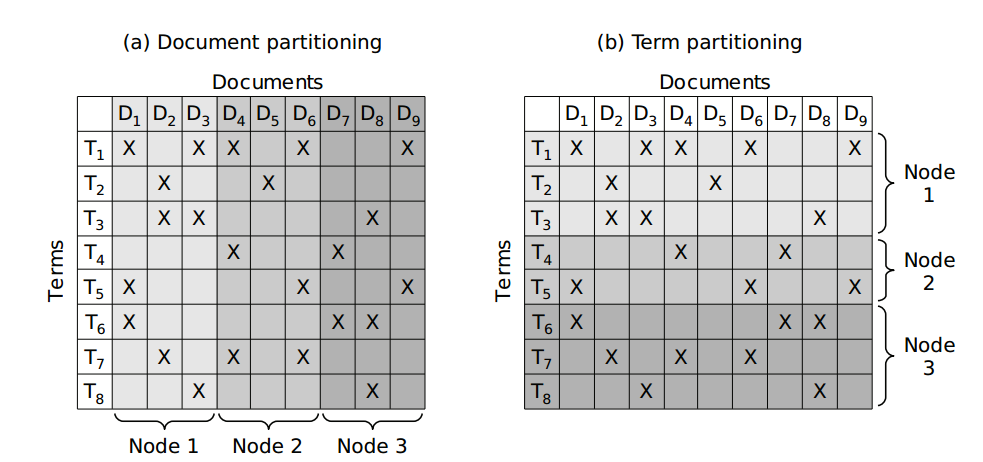
\includegraphics[scale=0.5]{imagens/particionamento-indice.png}
 \caption{Representação das duas abordagens de particionamento de índice}
\end{figure}

Assim, para resolver o problema da consulta durante a indexação são utilizados vários subíndices onde cada um tem um número máximo de documentos que podem ser indexados. Quando um subíndice atinge o número máximo de documentos ele está pronto para ser consultado. Tanto o número máximo de documentos por subíndice quanto a quantidade inicial de subíndices criados podem ser configurados pelo usuário por meio de argumentos de linha de comando.

\subsection{Arquitetura}

Alguns módulos utilizados na versão sequencial foram mantidos sem modificações, como foi o caso do \verb|Lexer|, \verb|Index| e \verb|Query|. Porém, para atender aos requisitos de paralelização, os demais módulos tiveram que ser modificados e outros tiveram que ser criados.

\begin{figure}[h]
 \centering
 \def\svgwidth{0.6\columnwidth}
 \input{arquitetura-paralelo.pdf_tex}
 \caption{Diagrama simplificado de como é feita a comunição entre threads}
\end{figure}

\textbf{Scanner}. Esse módulo teve que ser mudado para que a busca por documentos acontecesse em uma \emph{thread} separada. Assim, a descoberta de arquivos é executada paralelamente ao processamento e a indexação dos documentos. Esse comportamento caracteriza um modelo produtor-consumidor onde o \verb|Scanner| é o produtor, e as \emph{threads} de processamento e indexação são os consumidores. Tanto na versão Clojure como na versão Haskell esse modelo é implementado por meio de um \emph{buffer} compartilhado de capacidade infinita que bloqueia os consumidores que tentam ler do \emph{buffer} vazio até que novos elementos sejam produzidos.

\textbf{Engine}. Esse módulo é responsável pelo orquestramento das \emph{threads} de processamento e indexação de documentos e também das \emph{threads} de consulta. Inicialmente são criadas \emph{n} \emph{threads}\footnote{\emph{n} é fornecido pelo usuário} responsáveis pelo processamento e indexação dos documentos. Cada \emph{thread} executa em \emph{loop} enquanto houverem arquivos para serem processados. Esses arquivos são lidos do \emph{buffer} compartilhado com o \verb|Scanner|. Para cada arquivo que é lido, ele é processado, e em seguida indexado em um dos subíndices disponíveis. Após a indexação, se o subíndice estiver cheio (já tiver completado o número máximo de documentos por subíndice), ele é marcado como pronto e um novo subíndice vazio é adicionado à lista de subíndices disponíveis. Esse é o funcionamento das \emph{threads} de processamento e indexação. Já a parte das consultas funcionam da seguinta forma: sempre que um subíndice é marcado como pronto, uma nova \emph{thread} é criada para cada consulta fornecida pelo usuário. Cada \emph{thread} de consulta vai executar a consulta no subíndice e concatenar o resultado em uma variável transacional que é utilizada para acumular o resultado dessa consulta. Ao final, quando todos os subíndices tiverem sido consultados, cada variável transacional terá o resultado completo de uma consulta.

\textbf{Buffer}. Esse módulo abstrai o acesso aos \emph{buffers} que são compatilhados entre \emph{threads}. Contém funções para criação, adição e remoção de elementos.

\textbf{Logger}. É responsável por gerenciar o indicador de progresso do programa. Ele roda em uma \emph{thread} separada e fica recebendo mensagens de status dos demais módulos informando o progresso. Baseado nesses status as mensagens de indicação de progresso são formatadas e impressas no \emph{console} para o usuário durante a execução do programa.

\textbf{Main}. Como o controle do processamento dos arquivos e das consultas foi delegado ao módulo \verb|Engine|, o \verb|Main| na versão paralela apenas faz o \emph{parsing} dos parâmetros fornecidos pelo usuário e inicia o \verb|Scanner|, o \verb|Engine| e o \verb|Logger|.
\chapter{Resultados}

Para analisar o desempenho das implementações em Clojure e Haskell foi utilizada uma base de documento composta de 60 livros de domínio público em lingua inglesa que foram obtidos por meio do projeto Gutenberg\footnote{http://www.gutenberg.org/}, totalizando 36 \emph{megabytes} de arquivos texto. Foram utilizadas também seis consultas com tamanhos distintos e ocorrências variadas na base de documentos. Os experimentos foram executados em uma máquina com processador Intel Core i7-3770 3.4GHz com 4 núcleos físicos e 8 \emph{gigabytes} de memória RAM rodando Linux. Para o ambiente Haskell foi utilizado o compilador GHC 7.6.2 junto com a \emph{flag} de compilação \verb|-O|. Já para o ambiente Clojure foi utilizado Clojure 1.5.1 com OpenJDK 7.u17.

Todo o código produzido neste trabalho é aberto e está disponível junto com o histórico de desenvolvimento no GitHub\footnote{https://github.com/luisgabriel/tsearch}\footnote{https://github.com/luisgabriel/tsearch-clj}.

\begin{figure}[h]
 \centering
 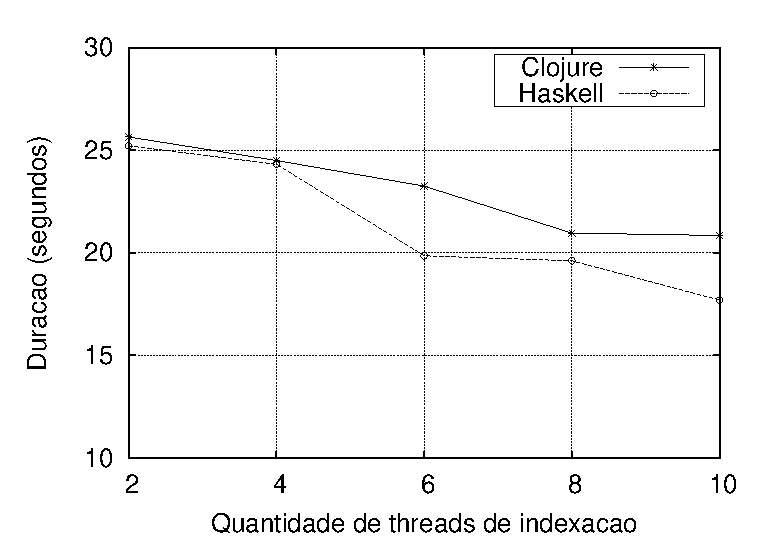
\includegraphics[scale=0.85]{imagens/clojure-haskell.eps}
 \caption{Gráfico do desempenho das versões paralelas em Clojure e Haskell}
 \label{fig:clj-hs-comp}
\end{figure}

A Figura \ref{fig:clj-hs-comp} mostra um gráfico onde o eixo horizontal representa a quantidade de \emph{threads} passada como argumento para o programa e o eixo vertical a duração em segundos da execução do programa. Cada ponto do gráfico representa a média do tempo de execução obtido a partir de 10 execuções consecutivas do programa calculado por meio do comando \verb|time| do Unix.

Como pode-se perceber, o desempenho de ambas as implementações foi bastante semelhante. As duas implementações se comportaram de maneira escalável durante os experimentos realizados, fazendo com que o aumento do número de \emph{threads} acarretasse em uma melhora do desempenho total do sistema.

\begin{figure}[!h]
 \begin{minipage}{0.5\textwidth}
  \centering
  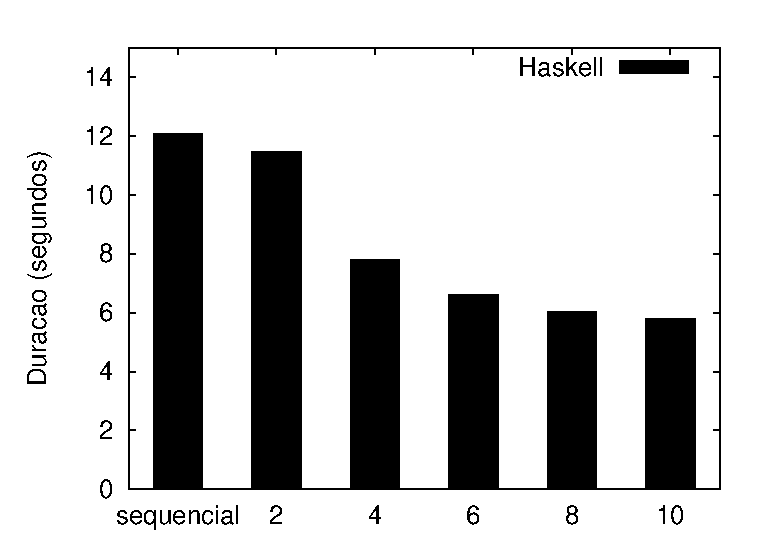
\includegraphics[scale=0.63]{imagens/haskell.eps}
 \end{minipage}
 \begin{minipage}{0.5\textwidth}
  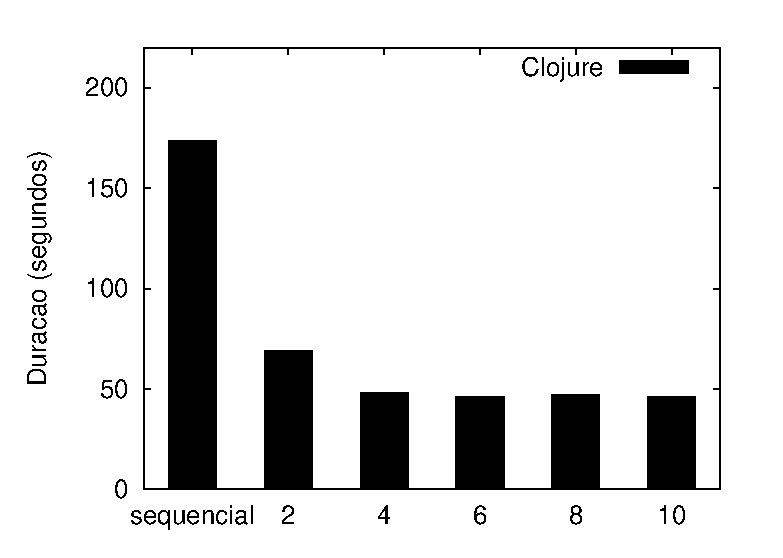
\includegraphics[scale=0.63]{imagens/clojure.eps}
 \end{minipage}
 \caption{Gráficos de comparação de desempenho entre das versões sequenciais e paralelas}
 \label{fig:clj-hs}
\end{figure}

A Figura \ref{fig:clj-hs}, por sua vez, mostra os mesmos dados do gráfico anterior com a adição dos resultados obtidos da execução dos mesmos experimentos com as implementações sequenciais em cada linguagem. Com esses gráficos pode-se notar que o principal objetivo da paralelização do problema foi alcançado já que a versão paralela, em todas as configurações testadas, conseguiu ter desempenho melhor que a versão sequencial.

\begin{figure}[!h]
 \begin{minipage}{0.5\textwidth}
  \centering
  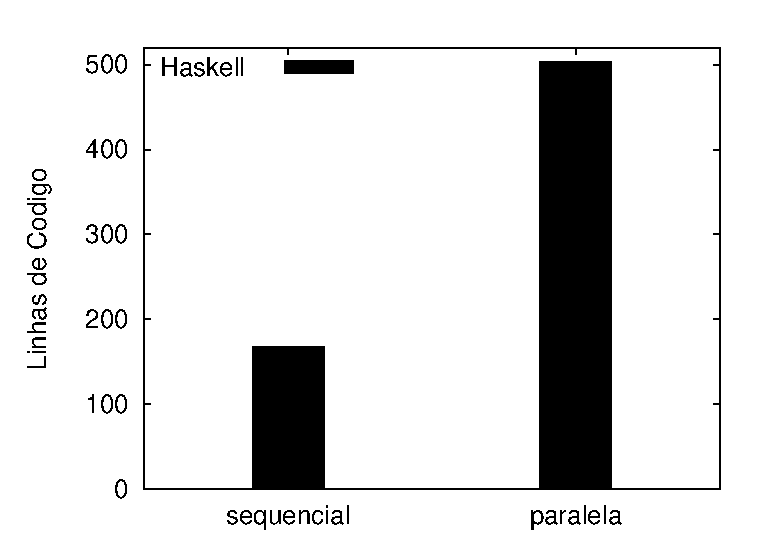
\includegraphics[scale=0.63]{imagens/loc-haskell.eps}
 \end{minipage}
 \begin{minipage}{0.5\textwidth}
  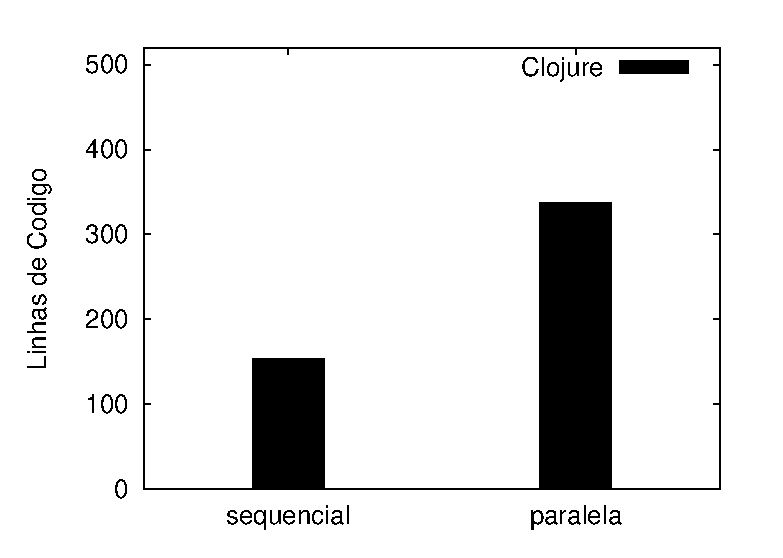
\includegraphics[scale=0.63]{imagens/loc-clojure.eps}
 \end{minipage}
 \caption{Gráficos de comparação da quantidade de linhas de código}
 \label{fig:clj-hs-loc}
\end{figure}

A Figura \ref{fig:clj-hs-loc} mostra o comparativo entre a quantidade de linhas de código total de todas as implementações. Como pode-se perceber, a paralelização implicou em um aumento considerável na quantidade de linhas de código dos projetos. No caso de Clojure, foi um aumento de aproximadamente 120\%, enquanto em Haskell foi um aumento de 200\%. Esse resultado mostra que, de fato, paralelizar um programa implica no aumento da complexidade da solução. Em um ambiente industrial, se faz necessário uma análise mais minuciosa para entender a relação de custo-benefício de se escrever sistemas concorrentes, pois, dependendo do cenário, melhorar o desempenho de um sistema em torno de 40\% ao custo de duplicar ou triplicar a base de código pode ser inaceitável.
\chapter{Conclusão}

Nesse trabalho foi apresentado como funciona e quais os requisitos necessário para implementação de um sistema Memória Transacional em Software, bem como a forma com que esse modelo é aplicado nas linguagens funcionais Clojure e Haskell. Por meio da implementação de um motor de busca paralelo, foi possível entender na prática como fazer uso de memória transacional para resolver um problema não trivial.

De uma forma geral, a utilização de memória transacional se mostrou como uma forma bastante natural de se lidar com memória compartilhada em um sistema concorrente. Agrupar um conjunto de operações para serem executadas de maneira atômica parece ser uma forma mais intuitiva de manter a consistência dos dados se comparado à proteção de accesso por meio da utilização de \emph{locks} e variáveis condicionais.

Também é importante notar que a utilização de linguagens funcionais para fins de implementação de sistemas concorrentes é algo bastante viável. Lidar com dados imutáveis isenta o desenvolvedor de muitas preocupações relacionadas à concorrência. E como foi mostrado no Capítulo 5, é possível organizar o código de maneira modularizada e se obter benefícios equiparáveis aos obtidos quando se desenvolve com linguagens orientadas à objetos em relação à modularidade do código.

As duas linguagens utilizadas nesse estudo, embora bastante distintas entre si, se mostraram muito flexíveis para o tipo de tarefa que foram utilizadas. Haskell tem a vantagem de ter um forte \emph{background} acadêmico que embasa grande parte das decisões de projeto da linguagem e reflete em mecanismos extremamente sofisticados e robustos como é o caso do seu sistema de tipos. Clojure, por sua vez, é uma linguagem que vem ganhando muito adeptos nos últimos anos e tem como principal vantagem a integração com a máquina virtual de Java, fazendo com que seja possível utilizar de uma gama de bibliotecas bastante atestadas de maneira muito simples através de uma integração fluída com a linguagem.

Em trabalhos futuros, o primeiro passo será realizar uma análise aprofundada da implementação do motor de busca em Clojure de forma que seja possível otimizá-lo para ter um desempenho equiparável à implementação feita em Haskell. Em seguida, para que as implementações atendam à todos os requisitos da especificação apresentada na Seção 5.1, os outros tipos de consulta serão implementados. A investigação de outros tipos de estruturas para representação do índice também podem ser explorados com a intenção de melhorar o desempenho das consultas e aumentar a concorrência (menos bloqueios) durante a indexação. Por fim, para fazer um estudo mais completo das implementações de STM de Clojure e Haskell seria interessante a utilização de um problema que envolvesse mais operações compostas e dependentes em sua regra de negócios como objeto de estudo.

%%
%% Parte pós-textual
%%
\backmatter

% Bibliografia
\nocite{*}
\bibliographystyle{IEEEtran}
\bibliography{bibliografia}

\end{document}
